% FiLM-TCN architecture as run in colab_benchmark_h1_h5.ipynb
% (--use_events --event_fusion channel --event_dim 16 --use_multi_scale False
%  --aggregate_horizon). Compile with pdflatex; include the PDF in the paper.
\documentclass[tikz,border=6pt]{standalone}
\usepackage{amsmath,amssymb}
\usetikzlibrary{positioning,arrows.meta,fit,calc}

\definecolor{cIO}{HTML}{98A8CE}
\definecolor{cRevIN}{HTML}{FFB3B8}
\definecolor{cStem}{HTML}{7FBFE0}
\definecolor{cConcat}{HTML}{A3ADDB}
\definecolor{cBlock}{HTML}{D79BDB}
\definecolor{cHead}{HTML}{AEF0EB}
\definecolor{cFiLM}{HTML}{7ED8A6}
\definecolor{cPast}{HTML}{DDF6F6}
\definecolor{cFut}{HTML}{CFCFCF}
\definecolor{cDrop}{HTML}{F6E7A8}

\begin{document}
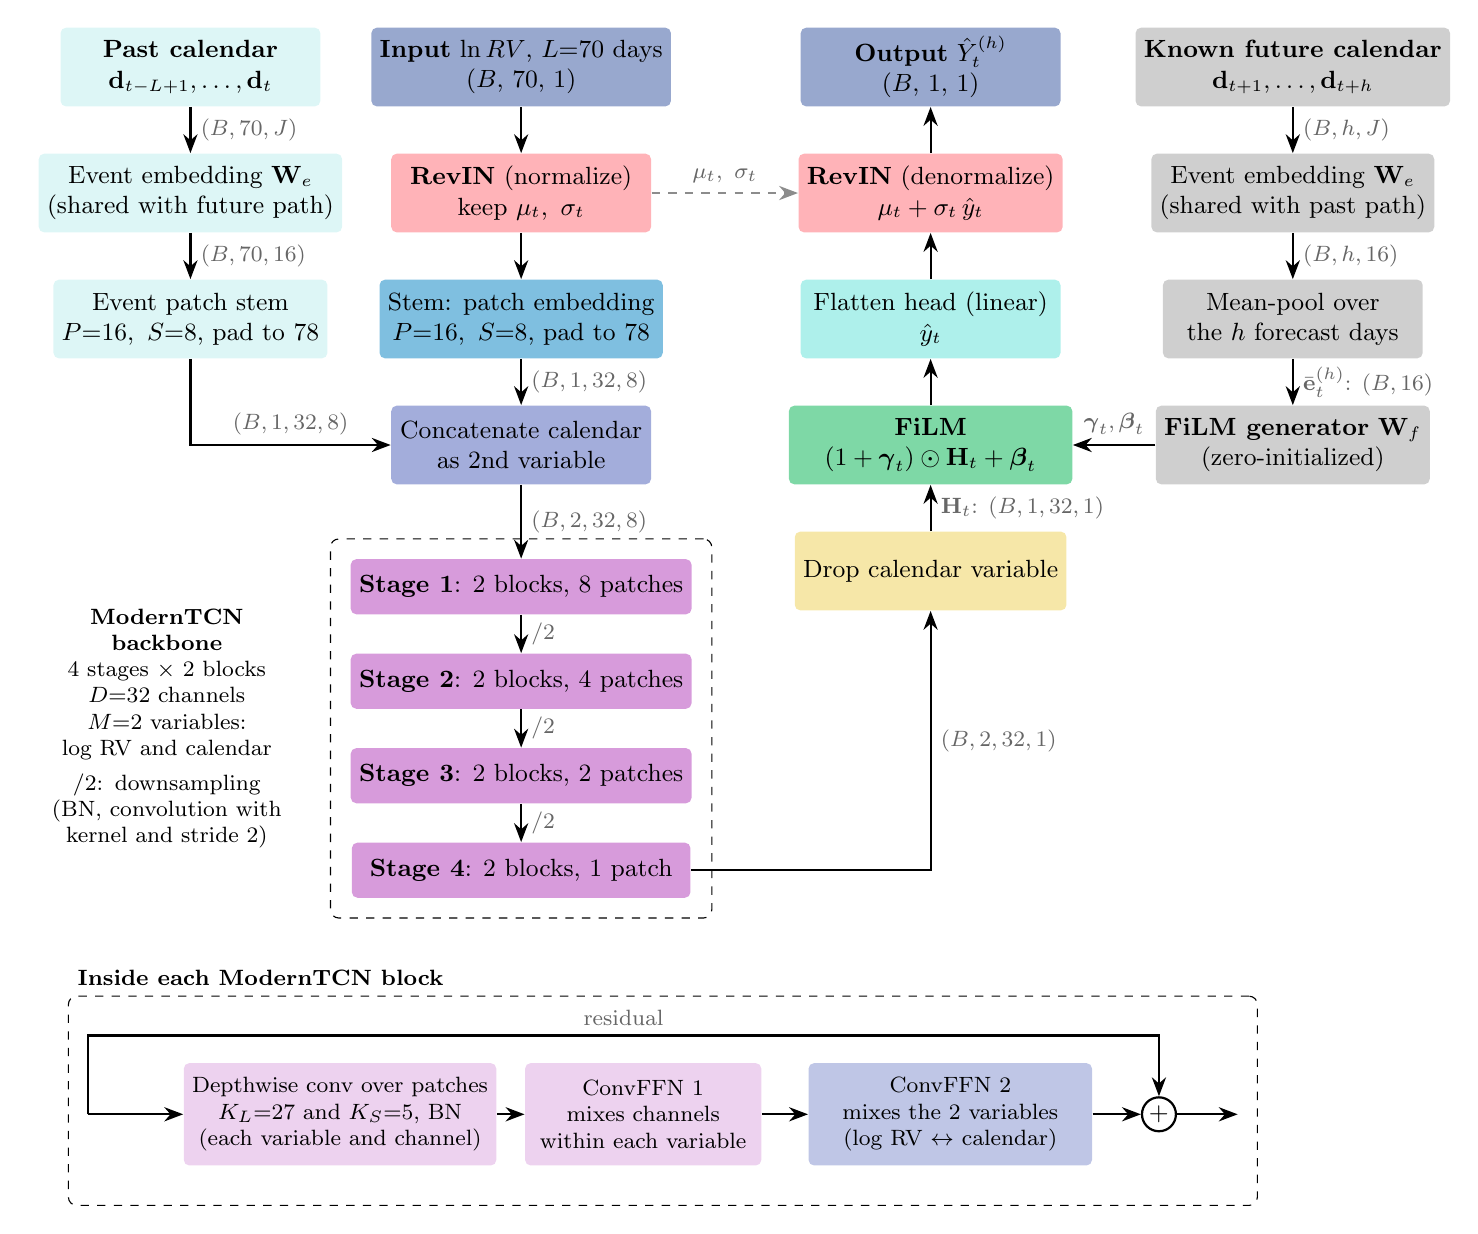
\begin{tikzpicture}[
  box/.style={rounded corners=2pt, minimum height=1.0cm, minimum width=3.3cm,
              align=center, font=\small, inner sep=3pt},
  stage/.style={box, fill=cBlock, minimum height=0.7cm, minimum width=4.3cm},
  arr/.style={-{Stealth[length=2.4mm,width=1.8mm]}, line width=0.8pt},
  dim/.style={font=\footnotesize, text=black!60},
  ibox/.style={rounded corners=2pt, minimum height=1.3cm, align=center,
               font=\footnotesize, inner sep=3pt},
]

% ---- past calendar path (look-back days) ---------------------------------
\node[box, fill=cPast] (p1) at (0,0)
  {\textbf{Past calendar}\\$\mathbf{d}_{t-L+1},\dots,\mathbf{d}_t$};
\node[box, fill=cPast] (p2) at (0,-1.6)
  {Event embedding $\mathbf{W}_e$\\(shared with future path)};
\node[box, fill=cPast] (p3) at (0,-3.2)
  {Event patch stem\\$P{=}16,\ S{=}8$, pad to 78};
\draw[arr] (p1) -- node[dim, right] {$(B,70,J)$} (p2);
\draw[arr] (p2) -- node[dim, right] {$(B,70,16)$} (p3);

% ---- value path -----------------------------------------------------------
\node[box, fill=cIO] (v1) at (4.2,0)
  {\textbf{Input} $\ln RV$, $L{=}70$ days\\$(B,\,70,\,1)$};
\node[box, fill=cRevIN] (v2) at (4.2,-1.6)
  {\textbf{RevIN} (normalize)\\keep $\mu_t,\ \sigma_t$};
\node[box, fill=cStem] (v3) at (4.2,-3.2)
  {Stem: patch embedding\\$P{=}16,\ S{=}8$, pad to 78};
\node[box, fill=cConcat] (v4) at (4.2,-4.8)
  {Concatenate calendar\\as 2nd variable};
\draw[arr] (v1) -- (v2);
\draw[arr] (v2) -- (v3);
\draw[arr] (v3) -- node[dim, right] {$(B,1,32,8)$} (v4);
\draw[arr] (p3) |- node[dim, pos=0.75, above] {$(B,1,32,8)$} (v4);

% ---- ModernTCN backbone: 4 stages x 2 blocks, downsampling between -------
\node[stage] (s1) at (4.2,-6.6)  {\textbf{Stage 1}: 2 blocks, 8 patches};
\node[stage] (s2) at (4.2,-7.8)  {\textbf{Stage 2}: 2 blocks, 4 patches};
\node[stage] (s3) at (4.2,-9.0)  {\textbf{Stage 3}: 2 blocks, 2 patches};
\node[stage] (s4) at (4.2,-10.2) {\textbf{Stage 4}: 2 blocks, 1 patch};
\draw[arr] (s1) -- node[dim, right] {$/2$} (s2);
\draw[arr] (s2) -- node[dim, right] {$/2$} (s3);
\draw[arr] (s3) -- node[dim, right] {$/2$} (s4);
\node[draw, dashed, rounded corners=3pt, fit=(s1)(s2)(s3)(s4),
      inner xsep=0.25cm, inner ysep=0.25cm] (bb) {};
\node[font=\footnotesize, align=center, text width=3.3cm] at (-0.3,-8.4)
  {\textbf{ModernTCN backbone}\\4 stages $\times$ 2 blocks\\
   $D{=}32$ channels\\$M{=}2$ variables:\\log RV and calendar\\[3pt]
   $/2$: downsampling\\(BN, convolution with\\kernel and stride 2)};
\draw[arr] (v4) -- node[dim, right] {$(B,2,32,8)$} (s1);

% ---- conditioning and output path ----------------------------------------
\node[box, fill=cDrop] (u1) at (9.4,-6.4) {Drop calendar variable};
\node[box, fill=cFiLM, minimum width=3.6cm] (u2) at (9.4,-4.8)
  {\textbf{FiLM}\\$(1+\boldsymbol{\gamma}_t)\odot\mathbf{H}_t+\boldsymbol{\beta}_t$};
\node[box, fill=cHead] (u3) at (9.4,-3.2)
  {Flatten head (linear)\\$\hat{y}_t$};
\node[box, fill=cRevIN] (u4) at (9.4,-1.6)
  {\textbf{RevIN} (denormalize)\\$\mu_t+\sigma_t\,\hat{y}_t$};
\node[box, fill=cIO] (u5) at (9.4,0)
  {\textbf{Output} $\hat{Y}_t^{(h)}$\\$(B,\,1,\,1)$};
\draw[arr] (s4.east) -| node[dim, right, pos=0.75] {$(B,2,32,1)$} (u1.south);
\draw[arr] (u1) -- node[dim, right] {$\mathbf{H}_t$: $(B,1,32,1)$} (u2);
\draw[arr] (u2) -- (u3);
\draw[arr] (u3) -- (u4);
\draw[arr] (u4) -- (u5);
\draw[arr, dashed, black!45] (v2) -- node[dim, above] {$\mu_t,\ \sigma_t$} (u4);

% ---- known future calendar (forecast days) -------------------------------
\node[box, fill=cFut] (f1) at (14.0,0)
  {\textbf{Known future calendar}\\$\mathbf{d}_{t+1},\dots,\mathbf{d}_{t+h}$};
\node[box, fill=cFut] (f2) at (14.0,-1.6)
  {Event embedding $\mathbf{W}_e$\\(shared with past path)};
\node[box, fill=cFut] (f3) at (14.0,-3.2)
  {Mean-pool over\\the $h$ forecast days};
\node[box, fill=cFut] (f4) at (14.0,-4.8)
  {\textbf{FiLM generator} $\mathbf{W}_f$\\(zero-initialized)};
\draw[arr] (f1) -- node[dim, right] {$(B,h,J)$} (f2);
\draw[arr] (f2) -- node[dim, right] {$(B,h,16)$} (f3);
\draw[arr] (f3) -- node[dim, right] {$\bar{\mathbf{e}}_t^{(h)}$: $(B,16)$} (f4);
\draw[arr] (f4) -- node[dim, above] {$\boldsymbol{\gamma}_t,\boldsymbol{\beta}_t$} (u2);

% ---- inside one ModernTCN block --------------------------------------------
\coordinate (bin) at (-1.3,-13.3);
\node[ibox, fill=cBlock!45, minimum width=3.5cm] (b1) at (1.9,-13.3)
  {Depthwise conv over patches\\$K_L{=}27$ and $K_S{=}5$, BN\\(each variable and channel)};
\node[ibox, fill=cBlock!45, minimum width=3.0cm] (b2) at (5.75,-13.3)
  {ConvFFN 1\\mixes channels\\within each variable};
\node[ibox, fill=cConcat!70, minimum width=3.6cm] (b3) at (9.65,-13.3)
  {ConvFFN 2\\mixes the 2 variables\\(log RV $\leftrightarrow$ calendar)};
\node[draw, circle, line width=0.8pt, inner sep=1pt, font=\small] (plus)
  at (12.3,-13.3) {$+$};
\coordinate (bout) at (13.3,-13.3);
\draw[arr] (bin) -- (b1);
\draw[arr] (b1) -- (b2);
\draw[arr] (b2) -- (b3);
\draw[arr] (b3) -- (plus);
\draw[arr] (plus) -- (bout);
\coordinate (rtop) at ($(bin)+(0,1.0)$);
\draw[arr] (bin) -- (rtop) -| node[dim, pos=0.25, above] {residual} (plus);
\node[draw, dashed, rounded corners=3pt, fit=(bin)(rtop)(b1)(b2)(b3)(plus)(bout),
      inner xsep=0.25cm, inner ysep=0.5cm,
      label={[font=\footnotesize\bfseries, anchor=south west]north west:%
             Inside each ModernTCN block}] {};

\end{tikzpicture}
\end{document}
